\documentclass{beamer}

\usepackage[ngerman]{babel}
\usepackage{graphicx} % fuer Bilder
\usepackage{listings} % fuer Code

\usetheme{Goettingen}

\lstset{language=C++} % fuer c++ code style

\title{Prozesslenkung: Hierarchische Zustandsautomaten II}
\subtitle{Implementierung Hierarchischer Zustandsautomaten}
\author{Katja Kirstein, Anne-Lena Kowalka, Marian Triebe, Eugen Winter}
\date{\today} 

\begin{document}
\begin{frame}
\titlepage
\end{frame}

%% Themen uebersicht
\begin{frame}
 \frametitle{Themen}
 \begin{itemize}
  \item Grundlagen GoF
  \item Externe Statevariablen
  \item Entry und Exit Code
  \item History
  \item Conditions/Guards/Choice Points
  \item Timer
 \end{itemize}
\end{frame}

%% GoF fsm Beispiel (Klassendiagramm)
\begin{frame}
 \frametitle{GoF State Pattern Struktur}
 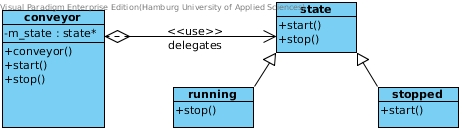
\includegraphics[scale=.6]{img/fsm_gof.jpg}
 \begin{itemize}
  \item Kontext-Klasse (conveyor)
  \item Zustands Basisklasse (state)
  \item Zust\"ande (running, stopped)
 \end{itemize}
\end{frame}

%% Grundlagen GoF
\begin{frame}
 \frametitle{Grundlagen GoF}
 Die klassiche GoF Implementierung hat einige schw\"achen
 \begin{itemize}
  \item Hoher Speicherverbrauch, da jeder State im Speicher gehalten werden muss, auch wenn diese eigentlich nicht verwendet werden
  \item Der h\"ohere Speicherverbrauch kann allerdings mit dem Placement New Operator umgangen werden
  \item Kontext muss eventuell immer mit \"ubergeben werden
 \end{itemize}
\end{frame}

%% GoF fsm Systemgrenzen
\begin{frame}
 \frametitle{Systemgrenzen}
\end{frame}

%% GoF fsm Automat
\begin{frame}
 \frametitle{Automat}
\end{frame}

%% GoF fsm States in Code I
\begin{frame}
 \frametitle{GoF States in Code I}
 \begin{itemize}
  \item Alle States erben von einer Oberstate Klasse
  \item Der Oberstate implementiert alle Events aller Zustände als leere virtuelle Funktion
  \item Der jeweilige Zustand implementiert nur seine eigenen Events, nicht relevante
  Events werden an die leeren Methoden der Basisklasse weitergereicht
 \end{itemize}
\end{frame}

%% GoF fsm States in Code (Header)
\begin{frame}[fragile]
 \frametitle{GoF States in Code (Header)}
 \begin{lstlisting}
  struct state {
    virtual ~state() { }
    virtual void start() { }
    virtual void stop() { }
  };

  struct running : public state {
    void stop();
  };

  struct stopped : public state {
    void start();
  };
 \end{lstlisting}
\end{frame}

%% GoF fsm States in Code (Implementierung/CPP)
\begin{frame}[fragile]
 \frametitle{GoF States in Code (Implementierung)}
 \begin{lstlisting}
  // transition running -> stopped
  void running::stop() {
    new (this) stopped;
    cout << "stop() / stop" << endl;
  }

  // transition stopped -> running
  void stopped::start() {
    new (this) running;
    cout << "start() / run" << endl;
  }
 \end{lstlisting}
\end{frame}

%% GoF fsm Kontext Klasse
\begin{frame}
 \frametitle{GoF Kontext Klasse}
 \begin{itemize}
  \item Sicht von au{\ss}en auf die FSM
  \item Dient als Delegator zu den States
  \item Bedient alle Eingangssignale durch Funktionen
 \end{itemize}
\end{frame}

%% GoF fsm Konext Klasse
\begin{frame}[fragile]
 \frametitle{GoF Kontext Klasse in Code}
 Header:
 \begin{lstlisting}
  struct conveyor {
    conveyor() : m_state(new stopped) { }
    ~conveyor() { delete m_state; }
    void start();
    void stop();
   private:
    state* m_state;
  };
 \end{lstlisting}
 Implementierung:
 \begin{lstlisting}
  void conveyor::start() {
    m_state->start();
  }
  void conveyor::stop() {
    m_state->stop();
  }
 \end{lstlisting}
\end{frame}

%% Schritte zum erstellen einer FSM
\begin{frame}
 \frametitle{Schritte zum erstellen einer FSM}
 \begin{enumerate}
  \item Erstellen der Systemgrenzen
  \item Erstellen einer FSM
  \item Umwandlung in Code
  \begin{itemize}
   \item Kontextklasse, Funktionsnamen als Eingangssignale
   \item Basisklasse für Zustände erstellen
   \item Zustandsklassen erben von der Basisklasse und implementieren nur die eigenen Reaktionen neu
  \end{itemize}
  \item Pr\"ufen ob Code und Systemgrenzen/Diagramm zusammenpassen
  \begin{itemize}
   \item Sind alle Eingangssignale als Funktionen zu finden?
   \item Werden alle Ausgangssignale verwendet/ausgegeben?
   \item Die Namen f\"ur Eingangssignale/Ausgangssignale sollten konsistent sein, da Fehler sonst vorprogrammiert!
  \end{itemize}
 \end{enumerate}
\end{frame}

%% Externe Statevariablen
\begin{frame}
 \frametitle{Externe Statevariablen}
\end{frame}

%% Entry und Exit Code
\begin{frame}
 \frametitle{Entry und Exit Code}
\end{frame}

%% History
\begin{frame}
 \frametitle{History}
\end{frame}

%% Conditions/Guards/Choice Points
\begin{frame}
 \frametitle{Conditions/Guards/Choice Points}
\end{frame}

%% Timer
\begin{frame}
 \frametitle{Timer}
\end{frame}

\end{document}